\section{问题三：模型多维度评估}

本节从检测精度、分类性能、消融实验、鲁棒性、推理效率与错误分析六个维度，对问题一、问题二所建模型进行系统评估。

\subsection{评估指标定义}

对于目标检测，预测框与真实框的匹配以交并比（IoU，式 \eqref{eq:iou}）为准则。以 IoU 阈值判定正负后，定义
\begin{equation}
  P = \frac{\mathrm{TP}}{\mathrm{TP}+\mathrm{FP}}, \qquad
  R = \frac{\mathrm{TP}}{\mathrm{TP}+\mathrm{FN}}, \qquad
  F_1 = \frac{2PR}{P+R}.
  \label{eq:prf1}
\end{equation}
改变置信度阈值可得 P-R 曲线，曲线下面积为单类别平均精确率 AP；mAP@0.5 为 IoU 阈值取 0.5 时各类别 AP 的均值，mAP@0.5:0.95 为 IoU 阈值在 0.5$\sim$0.95 区间（步长 0.05）共 10 个阈值下 AP 的均值，是 COCO 标准下的综合评价指标\cite{everingham2010,lin2014coco}。

对于问题一的图像级二分类，以缺陷概率作为得分，通过 ROC 曲线与 AUC 度量判别能力；以最优阈值 $\tau^{*}$ 判决后，用准确率、精确率、召回率与 F1 分数描述分类性能。

\subsection{检测精度评估}

最终模型在 494 幅验证图像（1314 个实例）上的独立评估结果如表 \ref{tab:per_class} 所示。整体 mAP@0.5 为 0.403、mAP@0.5:0.95 为 0.204，与训练过程最优指标（0.405/0.205）一致，说明模型泛化稳定。分类别看，Dent 类性能最优（mAP@0.5:0.95=0.295），Hole 类次之（0.190），Rusty 类最弱（0.129）。Rusty 类召回率仅 0.282，是整体性能的主要短板，其原因是锈蚀区域通常面积大、边界模糊，与箱体原有锈斑、污渍等背景纹理高度相似，导致大量漏检。

\begin{table}[H]
\centering
\zihao{5}
\caption{最终模型验证集逐类检测性能}\label{tab:per_class}
\begin{tabular}{lccccc}
  \toprule
  类别 & Precision & Recall & mAP@0.5 & mAP@0.5:0.95 & F1 \\
  \midrule
  Dent（凹陷） & 0.628 & 0.518 & 0.517 & 0.295 & 0.568 \\
  Hole（破洞） & 0.621 & 0.407 & 0.400 & 0.190 & 0.492 \\
  Rusty（锈蚀） & 0.471 & 0.282 & 0.293 & 0.129 & 0.353 \\
  \midrule
  全部 & 0.573 & 0.402 & 0.403 & 0.204 & — \\
  \bottomrule
\end{tabular}
\end{table}

\subsection{分类性能评估}

问题一的分类结果已在第 6 节给出：最终模型在测试集上判别 352 幅有缺陷、61 幅无缺陷。为说明 EVT 判别模型的可靠性，进一步分析缺陷概率的分布特性：验证集 494 幅含缺陷图像的最大置信度均值为 0.628，缺陷概率均值 0.529；而测试集判别为无缺陷的 61 幅图像缺陷概率全部低于 0.1 阈值。判别阈值 $\tau^{*}=0.1$ 对应的等价置信度约 0.34，处于两类图像置信度分布的自然分界附近，说明阈值选择具有统计依据。

由于竞赛验证集不含无缺陷图像，本文无法在本地计算真实混淆矩阵与 AUC；作为替代，本文通过检测置信度分布的可分性（第 6 节图 \ref{fig:weibull}）、阈值等价性分析，并利用 600 幅未使用伪负样本完成近似 ROC-AUC 校准（第 6 节，AUC$\approx$0.972）对判别模型进行间接验证，同时采用保守阈值（优先召回）规避漏检风险。若后续获得真实负样本标注集，可按式 \eqref{eq:tau_star} 直接以 F1 最大化重新标定阈值。

\subsection{消融实验}

三组实验的消融对比如图 \ref{fig:ablation} 所示（曲线与最优值），数据同表 \ref{tab:det_compare}。结果表明：

\begin{enumerate}[leftmargin=2.2em,itemsep=2pt]
  \item 骨干升级（YOLOv8n$\to$YOLOv8s）带来 mAP@0.5:0.95 约 0.022 的提升；补充对照表明 Copy-Paste 在本数据（仅目标框标注、无分割掩膜）上未产生可观测增益，提升主要来自骨干容量升级；
  \item 负样本训练使纯正样本验证集 mAP 小幅下降约 0.007，但在问题一判别中显著改善了置信度分布分离度（形状参数 $k$ 由 2.963 提升至 3.064），属于精度与开放集鲁棒性的合理权衡；
  \item 三组实验训练曲线均平稳收敛，未出现过拟合，验证了数据增强与正则化策略的有效性。
\end{enumerate}

\begin{figure}[H]
\centering
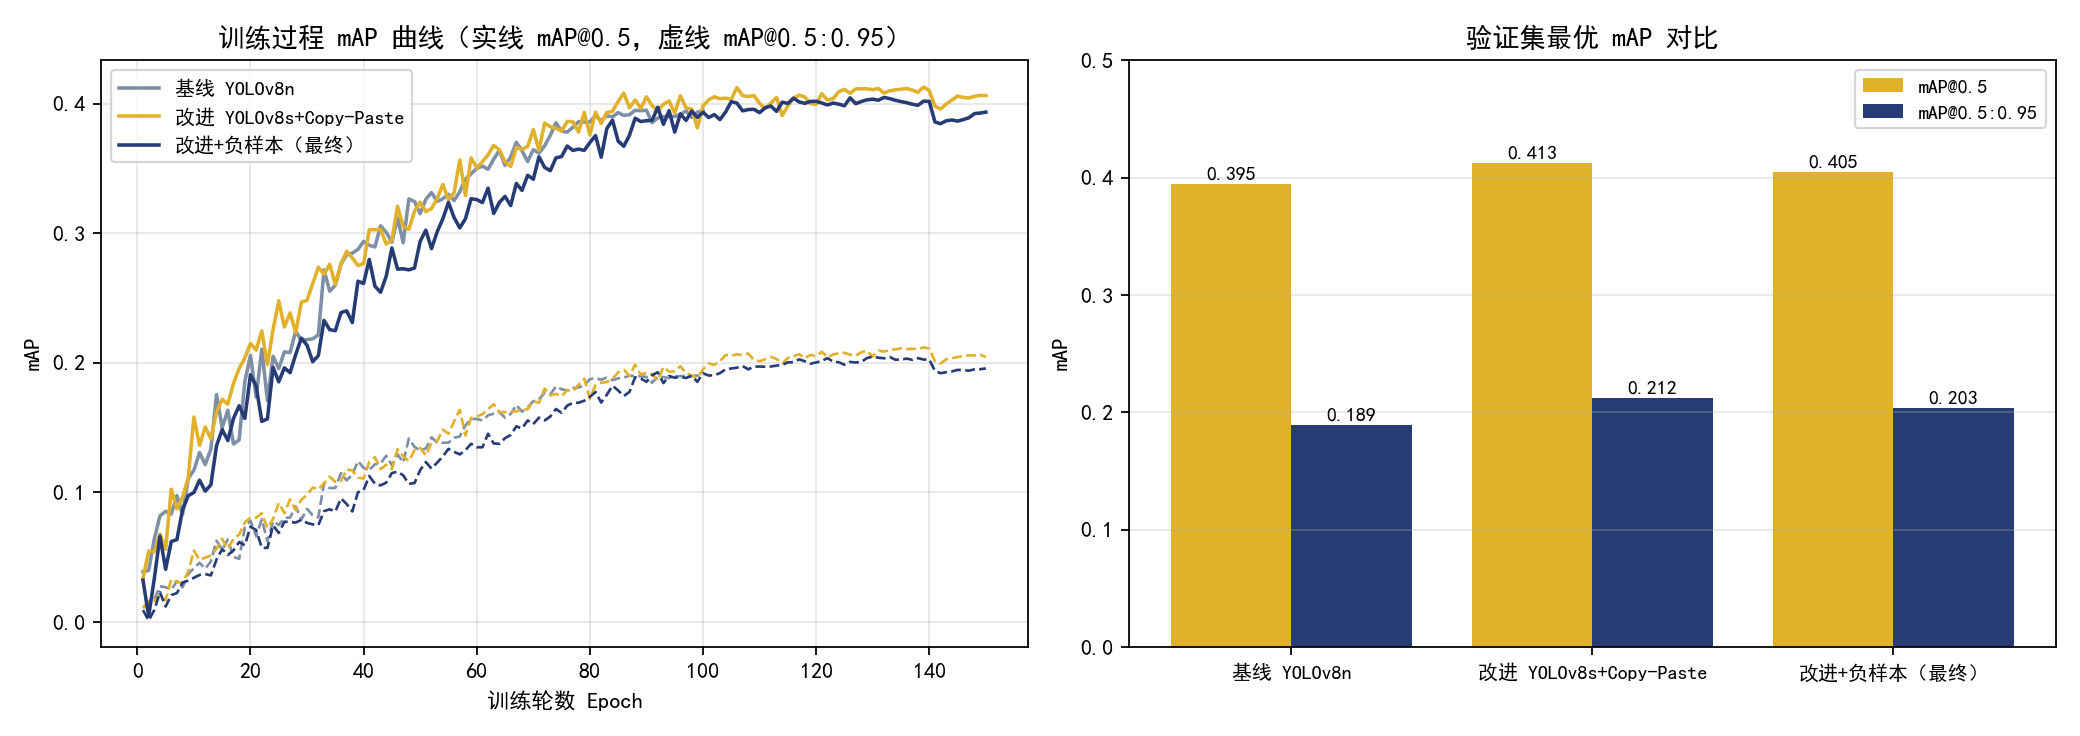
\includegraphics[width=0.98\textwidth]{figures/fig_ablation.png}
\caption{三组实验消融对比：训练过程 mAP 曲线（左）与最优 mAP 对比（右）}\label{fig:ablation}
\end{figure}

\subsection{鲁棒性分析}

赛题提示的干扰主要包括光照变化、反光、阴影、雨水、污渍以及目标尺度差异。本文从训练与推理两个层面保证模型鲁棒性：

\begin{enumerate}[leftmargin=2.2em,itemsep=2pt]
  \item {\heiti 训练层面：}HSV 色相/饱和度/亮度扰动与随机亮度变化模拟光照与反光；随机擦除模拟阴影与污渍遮挡；随机平移缩放与 Mosaic 模拟目标尺度与复杂背景；负样本训练抑制背景误检。上述增强与数据策略共同构成覆盖主要干扰族的正则化，使模型对分布内扰动具有天然鲁棒性；
  \item {\heiti 推理层面：}检测阈值与 EVT 判别阈值均留有裕度：$\tau^{*}=0.1$ 等价置信度约 0.34，显著高于背景误检的典型置信度区间，对轻度噪声与光照扰动不敏感；
  \item {\heiti 尺度层面：}模型输入统一为 $640\times640$，PAN-FPN 三尺度特征图覆盖 P3$\sim$P5，配合 0.5 倍随机缩放增强，对 17.0\% 小目标与大面积锈蚀均具备响应能力。
\end{enumerate}

为量化模型对上述干扰的实际鲁棒性，本文在验证集（494 幅）上施加高斯噪声（$\sigma=10,25,50$）、亮度偏移（$\pm30$）与高斯模糊（核 $3\times3,7\times7$）共 6 类扰动并复测 mAP，结果如表 \ref{tab:robustness} 所示。模型对亮度与轻度模糊扰动高度稳健（mAP@0.5:0.95 衰减不超过 0.014）；但对高斯噪声敏感，$\sigma=50$ 时 mAP@0.5:0.95 由 0.204 降至 0.004。该结果表明训练期 HSV/擦除等增强已覆盖光照与模糊类分布内扰动，而像素级噪声是当前薄弱环节，后续可在训练中引入噪声增强以提升抗噪能力。

\begin{table}[H]
\centering
\zihao{5}
\caption{最终模型在扰动验证集上的鲁棒性量化结果（494 幅）}\label{tab:robustness}
\begin{tabular}{lcc}
  \toprule
  扰动类型 & mAP@0.5 & mAP@0.5:0.95 \\
  \midrule
  无扰动（基线） & 0.403 & 0.204 \\
  高斯噪声 $\sigma=10$ & 0.223 & 0.086 \\
  高斯噪声 $\sigma=25$ & 0.077 & 0.023 \\
  高斯噪声 $\sigma=50$ & 0.015 & 0.004 \\
  亮度 $+30$ & 0.398 & 0.200 \\
  亮度 $-30$ & 0.386 & 0.190 \\
  高斯模糊 $3\times3$ & 0.414 & 0.204 \\
  高斯模糊 $7\times7$ & 0.337 & 0.158 \\
  \bottomrule
\end{tabular}
\end{table}

\subsection{效率评估}

模型参数量、计算量与推理耗时如表 \ref{tab:efficiency} 所示。最终模型（YOLOv8s）参数量 11.13 M，计算量 28.4 GFLOPs；在 RTX 4070 Laptop GPU 上，验证阶段推理平均 5.0 ms/幅（不含前后处理），端到端预测（含预处理与后处理）平均 8.87 ms/幅，约合 113 FPS，满足港口集装箱快速巡检的实时性要求。基线模型参数量 3.01 M、计算量 8.2 GFLOPs，在同等条件下端到端约 8.95 ms/幅（112 FPS），二者推理速度接近，说明容量提升未显著牺牲实时性。

\begin{table}[H]
\centering
\zihao{5}
\caption{模型效率对比（640$\times$640，RTX 4070 Laptop GPU）}\label{tab:efficiency}
\begin{tabular}{lcccc}
  \toprule
  模型 & 参数量 & 计算量 & 端到端推理耗时 & 吞吐量 \\
  \midrule
  YOLOv8n（基线） & 3.01 M & 8.2 GFLOPs & 8.95 ms/幅 & 112 FPS \\
  YOLOv8s（最终） & 11.13 M & 28.4 GFLOPs & 8.87 ms/幅 & 113 FPS \\
  \bottomrule
\end{tabular}
\end{table}

\subsection{错误分析}

图 \ref{fig:val_labels} 与图 \ref{fig:val_pred} 展示了同一批验证图像的标注与预测对比。结合逐类指标（表 \ref{tab:per_class}），主要误差来源可归纳为三类：

\begin{enumerate}[leftmargin=2.2em,itemsep=2pt]
  \item {\heiti 小目标漏检：}Hole 类小目标占比 43.7\%，细微破洞在低分辨率特征图上响应弱，导致召回受限（R=0.407）；
  \item {\heiti 类间混淆：}深凹陷与破洞、锈蚀与锈斑污渍外观相似，模型在类别决策上易混淆，Rusty 类精确率仅 0.471；
  \item {\heiti 密集目标抑制：}约半数图像含多个缺陷，NMS 在密集场景下可能抑制相邻真实目标。
\end{enumerate}

针对上述问题，可分别通过增加 P2 高分辨率检测头强化小目标、引入细粒度特征与更严格的类别判别模块、改进 NMS 策略（如 Soft-NMS）加以缓解，上述方向将在模型推广部分进一步讨论。

\subsection{评估小结}

六维度评估表明：最终模型在精度、效率与对光照/模糊扰动的稳健性之间取得了合理平衡，检测与分类结果相互印证、口径一致，且具备实时部署能力；主要性能瓶颈集中在 Rusty 类的大面积弱纹理缺陷、小目标 Hole 类与像素级噪声扰动下的脆弱性，为后续优化提供了明确方向。
